% Relazione del progetto di Visual Analytics (602AA) - VAST Challenge 2025, Mini-Challenge 3
% Compilazione: tectonic relazione_it.tex (oppure pdfLaTeX). Le figure sono in ../docs/screenshots/ e ../docs/mockups/.
\documentclass[11pt,a4paper]{article}

\usepackage[utf8]{inputenc}
\usepackage[T1]{fontenc}
\usepackage[italian]{babel}
\usepackage[a4paper,margin=2.3cm]{geometry}
\usepackage{lmodern}
\usepackage{microtype}
\usepackage{booktabs}
\usepackage{tabularx}
\usepackage{graphicx}
\graphicspath{{../docs/screenshots/}{../docs/mockups/}{fig/}}
\usepackage{enumitem}
\usepackage{caption}
\usepackage{float}
\usepackage[hidelinks]{hyperref}

\setlist{leftmargin=1.4em,itemsep=2pt,topsep=3pt}
\captionsetup{font=small,labelfont=bf}
\renewcommand{\arraystretch}{1.15}

\begin{document}

\begin{titlepage}
\centering
\vspace*{3cm}
{\large Visual Analytics\par}
\vspace{0.4cm}
{\normalsize Università di Pisa\par}
\vspace{2.5cm}
{\huge\bfseries Project Report\par}
\vspace{0.8cm}
{\large Analisi delle comunicazioni radio di Oceanus\par}
\vspace{0.2cm}
{\large VAST Challenge 2025, Mini-Challenge 3\par}
\vfill
{\normalsize Studente: Giuseppe Vincenzo Dylan Toscano (599752)\par}
\vspace{0.4cm}
{\normalsize Anno Accademico 2025--2026\par}
\vspace*{2.5cm}
\end{titlepage}

\tableofcontents
\newpage

%---------------------------------------------------------------------
\section{Introduzione}
%---------------------------------------------------------------------
Il progetto propone una soluzione alla Mini-Challenge 3 della VAST Challenge 2025, ambientata sull'isola di
Oceanus. Il giornalista Clepper Jensen ha registrato per due settimane (1--14 ottobre 2040) le comunicazioni radio
intercettate sull'isola e, con l'aiuto di uno stagista, ne ha ricavato un knowledge graph con gli eventi e le
relazioni tra le persone coinvolte. Nei messaggi si parla soprattutto di Nemo Reef, un'area marina protetta la
cui chiusura viene annunciata il 10 ottobre, mentre sull'isola si prepara un evento della cantante Sailor Shift.

Le domande della challenge sono quattro:
\begin{enumerate}
  \item quali sono i ritmi giornalieri delle comunicazioni, come cambiano tra le due settimane e quali entità
        influenzano un'entità scelta;
  \item quali gruppi di persone e barche si possono individuare e di quali argomenti parla ciascun gruppo;
  \item chi usa pseudonimi (Boss, The Middleman, Mrs.\ Money e altri) e chi c'è dietro;
  \item se Nadia Conti, in passato coinvolta in un giro di pesca illegale, sta continuando a svolgere attività illecite.
\end{enumerate}

L'obiettivo è costruire un'interfaccia che permetta al giornalista di rispondere da solo a queste domande.
Il giornalista conosce bene il contesto ma non è esperto di grafi. Per questo ho evitato di mostrare il grafo
intero come un groviglio di nodi e archi, e da ogni elemento grafico si può arrivare al testo dei messaggi da
cui deriva, che per lui sono la vera prova.

Tutti i grafici sono realizzati in D3.js, compresa la vista originale richiesta dal corso
(sezione~\ref{sec:orig}). Le pagine e i filtri sono gestiti con Vue.js e lo stile con Tailwind CSS; la
preparazione dei dati è fatta in Python (pandas e networkx). Il repository contiene la preparazione dei dati
(\texttt{scripts/}), l'applicazione (\texttt{app/}) e il notebook di esplorazione con i mockup
(\texttt{analysis/}, \texttt{docs/}); le istruzioni per avviare l'applicazione sono nel file
\texttt{README.md}. I dati della challenge non sono inclusi e vanno scaricati dal sito della VAST Challenge.

%---------------------------------------------------------------------
\section{Comprensione e preparazione dei dati}
%---------------------------------------------------------------------
\subsection{Struttura del grafo}
Il file \texttt{MC3\_graph.json} è un grafo orientato con 1159 nodi e 3226 archi. I nodi sono di tre tipi:
72 entità (persone, barche, organizzazioni, luoghi, gruppi), 802 eventi, di cui 584 sono comunicazioni radio,
e 285 nodi relazione. Le relazioni sono reificate: una relazione tra due entità (per esempio
\emph{Colleagues} o \emph{Operates}) è un nodo collegato alle due entità, e gli archi \texttt{evidence\_for}
collegano i messaggi alle relazioni che sostengono. Gli archi \texttt{sent} e \texttt{received} indicano
mittente e destinatario di ogni messaggio secondo i metadati della radio.

Per l'analisi il grafo è stato trasformato in tabelle: una tabella dei messaggi (mittente, destinatario, data,
testo), una delle relazioni tra coppie di entità e una delle prove che collegano messaggi e relazioni. Dopo
la pulizia restano 581 messaggi (sono stati tolti 3 duplicati esatti), scambiati da 40 attori (17 persone,
14 barche, 5 organizzazioni e 4 luoghi), e 192 relazioni tra questi attori, ognuna con l'elenco dei messaggi
che la sostengono.

I messaggi coprono tutti i 14 giorni, con 34--49 messaggi al giorno, e sono inviati solo tra le 8 e le 15,
con un picco alle 10 (146 messaggi). Questa è anche la fascia oraria mostrata nel calendario della prima
pagina.

\subsection{Mittente registrato e mittente reale}\label{sec:mittenti}
Quasi tutti i messaggi iniziano con una formula di chiamata del tipo ``Davis, Mako here'', da cui si capisce
che Mako sta scrivendo a Davis. Queste formule sono state riconosciute in 569 messaggi su 584 e confrontate con
il mittente e il destinatario registrati dalla radio. Il confronto ha dato questi risultati:
\begin{itemize}
  \item in 80 messaggi il grafo riporta un mittente o un destinatario diverso da quello del testo: in 76 è
        sbagliato il mittente e in 4 solo il destinatario;
  \item dei 76 messaggi con il mittente sbagliato, 43 hanno mittente e destinatario invertiti e 31 risultano
        inviati a sé stessi (per esempio Davis $\rightarrow$ Davis con il testo ``Davis, Mako here''). In tutti
        questi 74 casi la radio ha registrato il destinatario al posto del mittente;
  \item rimangono 2 messaggi in cui la differenza non si spiega in questo modo; vengono discussi nella
        sezione~\ref{sec:q3}.
\end{itemize}
In un primo momento avevo interpretato le firme diverse dal mittente come possibili pseudonimi. Il numero
anomalo di messaggi inviati a sé stessi mi ha portato a ricontrollare i testi, e si è visto che nella
maggior parte dei casi era la radio ad aver registrato male chi aveva inviato il messaggio. Questo passaggio è importante per la terza domanda, perché altrimenti si sarebbero
cercati pseudonimi che non esistono. Per ogni messaggio vengono comunque conservati sia i valori corretti
sia quelli originali della radio, e nell'interfaccia è possibile tornare ai dati originali.

\subsection{Dati derivati}
Sopra le tabelle sono stati calcolati alcuni dati aggiuntivi:
\begin{itemize}
  \item \textbf{Gruppi}: calcolati con l'algoritmo di Louvain, che mette nello stesso gruppo gli attori che
        si scambiano molti messaggi tra loro e pochi con gli altri. Ho dato a ogni gruppo il nome di un membro
        conosciuto o di quello che fanno:
        Operazione Nemo Reef (15 attori, tra cui Nadia Conti, Davis e le barche Mako e Remora), Controllo e
        istituzioni (15 attori, tra cui l'Oceanus City Council, i porti, i Green Guardians e le barche di
        sorveglianza), Alias (gli 8 pseudonimi) e Investigatori (Clepper Jensen e Miranda Jordan).
  \item \textbf{Temi}: dieci temi individuati con parole chiave, per esempio \emph{permessi} (``permit'',
        ``authoriz'', ``clearance''), \emph{soldi / pagamenti}, \emph{attrezzature / lavori} e
        \emph{segretezza}. Un messaggio può avere più temi. È un metodo approssimativo, ma le regole sono
        semplici da controllare e per ogni tema si possono leggere i messaggi trovati.
  \item \textbf{Orari citati}: le ore scritte nel testo dei messaggi (per esempio ``meet at 0500'' o
        ``7PM''), in tutto 169.
  \item \textbf{Azioni sospette}: leggendo i messaggi di Nadia Conti e di Boss ho segnato a mano 24 azioni
        sospette (18 di Nadia e 6 di Boss), divise in sei tipi, più una prova contraria. Ogni azione è collegata
        al messaggio da cui deriva, quindi può essere verificata.
\end{itemize}

%---------------------------------------------------------------------
\section{Progettazione e funzionamento dell'interfaccia}
%---------------------------------------------------------------------
\subsection{Stato dell'arte}
Il modo più comune di mostrare un knowledge graph è disegnarlo tutto come nodi e archi, con le posizioni
calcolate da un algoritmo a forze. Con 40 attori e alcune centinaia di collegamenti il risultato è un groviglio
difficile da leggere, soprattutto per chi non è esperto di grafi. Ho preferito quindi viste che aggregano i dati
e mettono il tempo su un asse (calendario, timeline), un grafo diviso in zone, una per gruppo, e, per
confrontare due versioni dello stesso dato, un grafico a nastri che collega due liste di nomi. Il problema
tipico di questa challenge, cioè i mittenti registrati in modo sbagliato, non basta mostrarlo: serve anche un
modo per scegliere quale versione usare e vedere cosa cambia nel resto dell'analisi, ed è da qui che nasce la
vista originale (sezione~\ref{sec:orig}).

\subsection{Modello e schema di comunicazione}
L'interfaccia ha una pagina per ogni domanda della challenge, e in cima a ogni pagina è scritta la domanda a
cui risponde. Ogni pagina si legge nello stesso ordine: prima i grafici con il quadro generale, poi i filtri
per restringere, infine il testo dei singoli messaggi quando si clicca un elemento. L'utente può esplorare
liberamente, ma ci sono alcuni punti di partenza già impostati: per esempio la prima e la quarta pagina si aprono con Nadia Conti già
selezionata.

Una barra comune in alto contiene la navigazione tra le pagine, il campo per scegliere un attore e i filtri
per gruppo, periodo (14 giorni, prima settimana, seconda settimana) e tema, con il numero di messaggi
selezionati. L'attore e i filtri valgono in tutte le pagine, e cliccando un attore in una vista lo si sceglie
anche nelle altre. A destra c'è sempre il pannello dei messaggi: cliccando un elemento di un grafico (una
lineetta, una barra, una cella, un arco o un nastro) il pannello mostra il testo dei messaggi che stanno dietro
a quell'elemento.

\subsection{Scelte di design: colori, forme e interazioni}
\paragraph{Colori.} Il colore identifica il gruppo dell'attore ed è lo stesso in tutte le viste: arancione per
Operazione Nemo Reef, verde per Controllo e istituzioni, rosa per gli Alias e blu per gli Investigatori. Sono
colori della palette Okabe-Ito, scelta perché resta distinguibile anche per chi è daltonico. Per le quantità, come
nella tabella dei temi, si usa la scala magma invertita, che va dal chiaro allo scuro; viridis è stata scartata
perché il suo verde è troppo simile a quello di Controllo e istituzioni. Le due settimane usano lo stesso
viola con due luminosità, perché sono un dato ordinato. Il grigio è usato solo per sfondi e contesto, mai per
una quantità. I testi colorati sono stati scuriti fino ad avere un contrasto di almeno 4,5:1 con lo sfondo.

\paragraph{Forme e codifiche.} Il tipo di attore è indicato dalla forma del simbolo: cerchio per le persone,
triangolo per le barche, quadrato per le organizzazioni, rombo per i luoghi. Le quantità da confrontare sono
mostrate come posizione su una scala comune o come lunghezza di barre che partono da zero, perché sono le
codifiche che si leggono con più precisione (classifica di Cleveland e McGill). L'area è usata solo per la dimensione dei
nodi nel grafo, dove basta capire chi è più attivo. Gli elementi meno certi sono resi più chiari o vuoti: per
esempio le relazioni sostenute da un solo messaggio o le azioni riferite da altri.

\paragraph{Titoli.} Il titolo di ogni grafico descrive quello che il grafico mostra, per esempio ``Il giorno
più fitto è l'11 ottobre (49 messaggi): chiusura Nemo Reef''. I titoli sono calcolati dai dati visualizzati,
quindi cambiano insieme ai filtri e all'attore scelto. La spiegazione di come leggere ogni grafico è nel
simbolo \textsf{i} accanto al titolo.

\paragraph{Interazioni.} Tutti i grafici hanno un tooltip al passaggio del mouse. Il clic su un elemento apre i
messaggi corrispondenti nel pannello a destra; il clic su un attore lo seleziona in tutte le pagine e lo
evidenzia nelle viste. Nel grafo della seconda pagina si può fare zoom con la rotella, nel calendario si può
cliccare un giorno per ingrandirlo.

\subsection{Struttura dell'interfaccia}
\subsubsection{Q1: ritmi e influenze}
\begin{figure}[!htbp]\centering
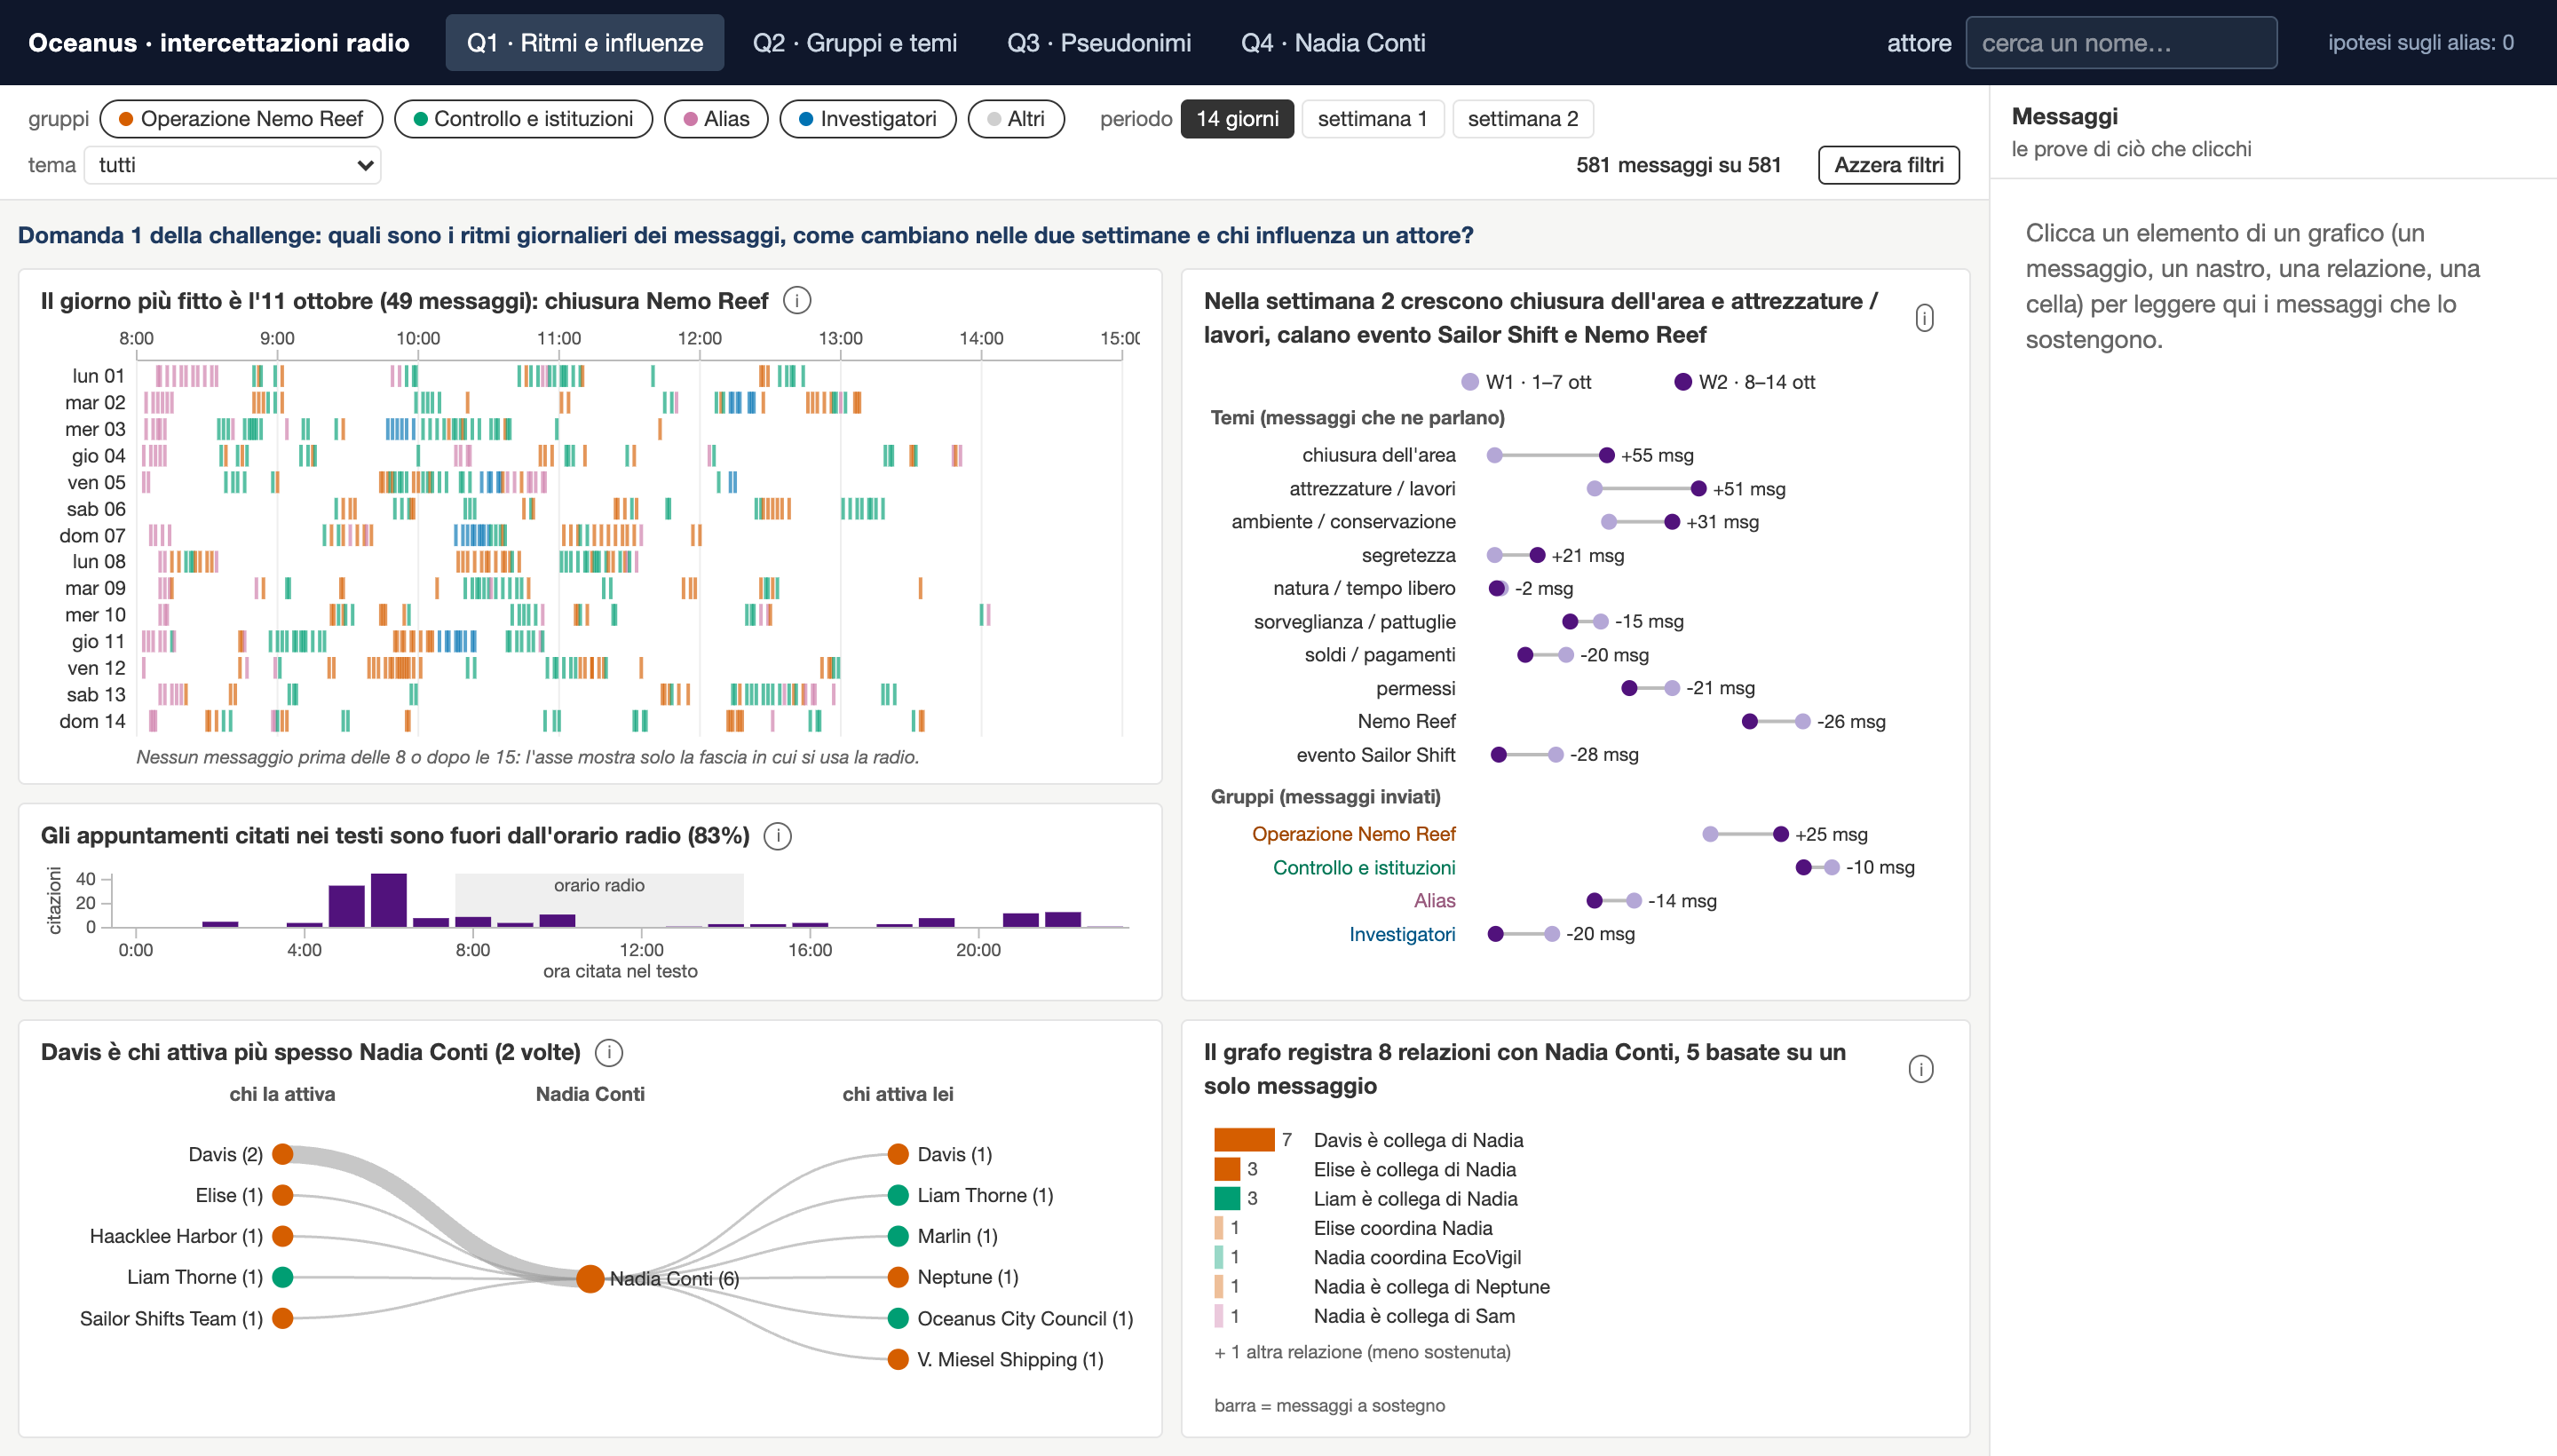
\includegraphics[width=\linewidth]{01_q1_ritmi.png}
\caption{Prima pagina: calendario dei messaggi e orari citati nei testi (a sinistra), confronto tra le due
settimane (a destra), chi attiva l'attore scelto e le sue relazioni nel grafo (in basso).}\label{fig:p1}
\end{figure}
Il widget principale è un calendario con una riga per giorno e l'orario sull'asse orizzontale (dalle 8 alle 15).
Ogni messaggio è una lineetta colorata in base al gruppo di chi lo invia. Avevo considerato una heatmap con
celle di un'ora, ma l'aggregazione nascondeva le sequenze di messaggi a pochi minuti di distanza, che in questo
dataset sono frequenti. Sotto il calendario c'è un grafico a barre con gli orari citati nei testi, sulle 24 ore,
con la fascia di uso della radio evidenziata in grigio.

A destra, un grafico a manubrio (dumbbell) confronta la prima e la seconda settimana per ogni tema e per ogni
gruppo, sulla stessa scala; le righe sono ordinate dall'aumento più grande e accanto è scritta la differenza
(per esempio ``+55 msg''). In basso ci sono due widget legati all'attore scelto. Il primo mostra a sinistra chi
gli scrive poco prima che lui scriva a qualcun altro (entro 15 minuti) e a destra a chi scrive subito dopo, con
lo spessore proporzionale al numero di volte. È una misura di precedenza nel tempo e non dimostra un rapporto
di comando. Il secondo elenca le relazioni che il grafo registra per l'attore, scritte come frasi (``Davis
è collega di Nadia'') e con il numero di messaggi che le sostengono.

\subsubsection{Q2: gruppi e temi}
\begin{figure}[!htbp]\centering
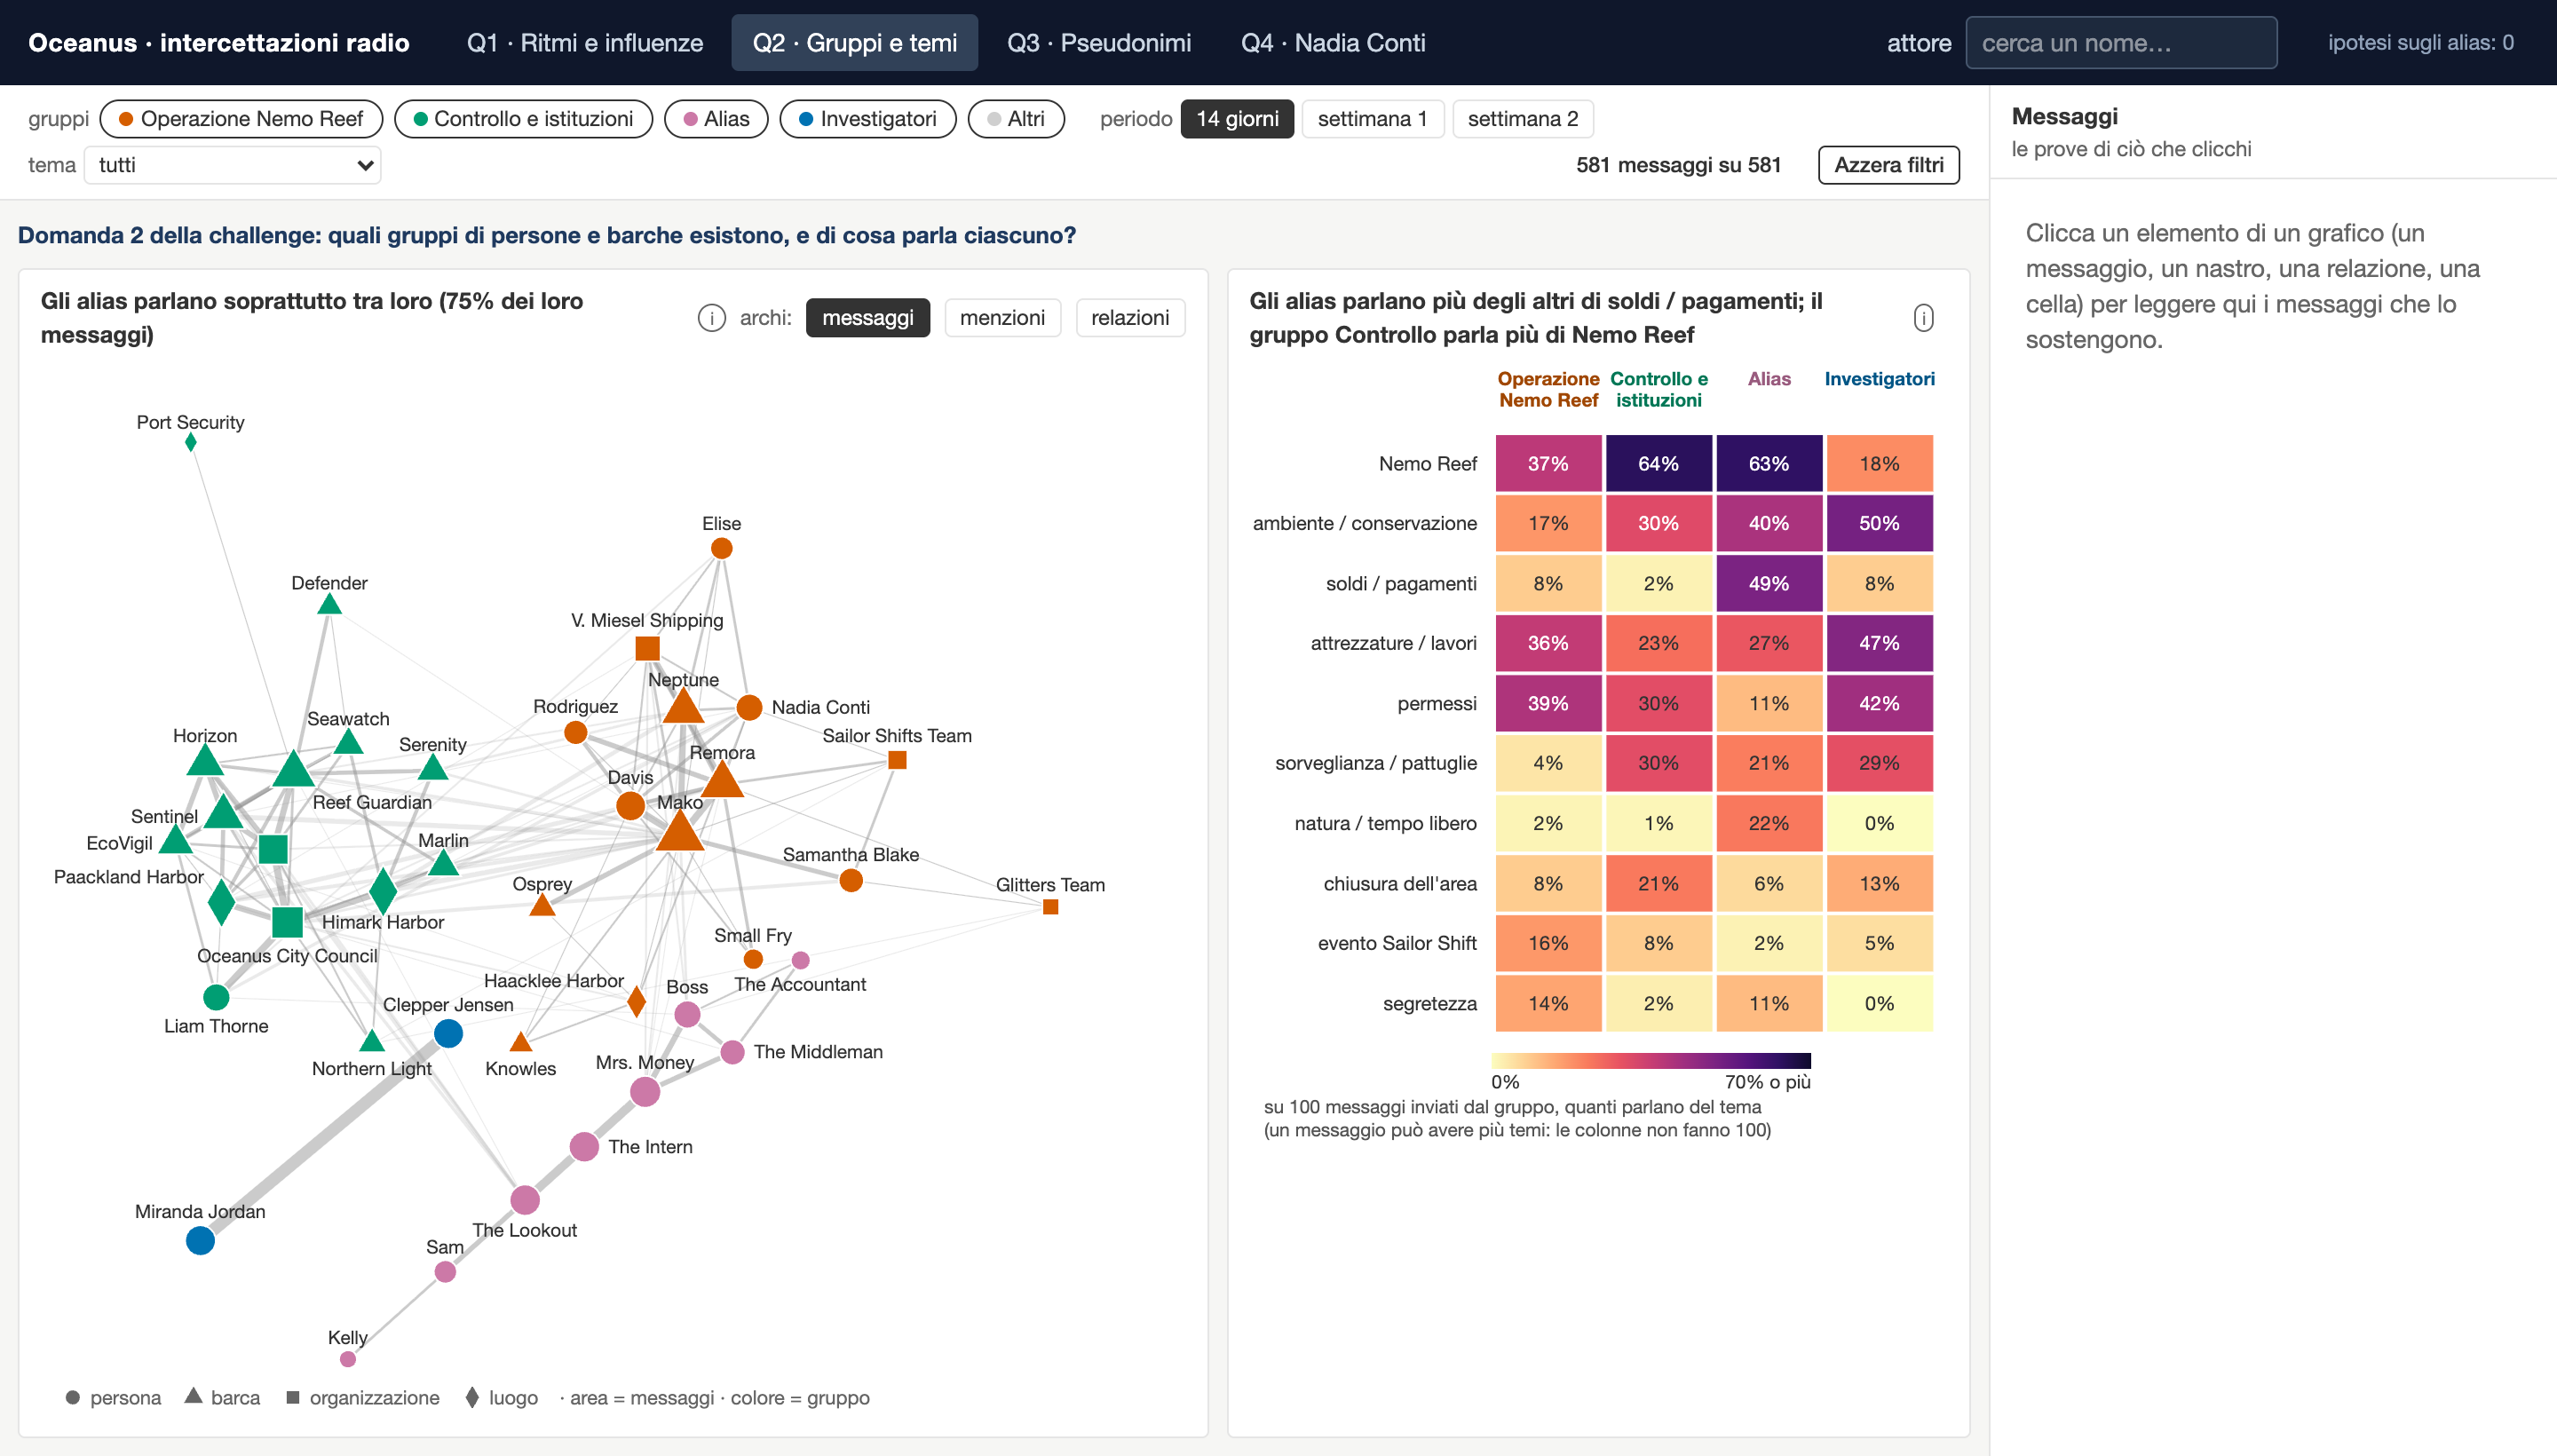
\includegraphics[width=\linewidth]{07_q2_gruppi_messaggi.png}
\caption{Seconda pagina: il grafo degli attori con una zona per gruppo e la tabella dei temi per gruppo.}\label{fig:p2}
\end{figure}
Il grafo mostra i 40 attori divisi in quattro zone, una per gruppo, e i nodi restano sempre nella stessa
posizione. Con un pulsante si sceglie quali collegamenti disegnare sugli stessi nodi: i messaggi scambiati, le menzioni nel testo e le relazioni del grafo.
I collegamenti tra gruppi diversi sono più chiari di quelli interni, così si vedono prima i blocchi; i nomi
vengono posizionati in modo da non sovrapporsi. La tabella accanto ha i temi sulle righe e i gruppi sulle
colonne; ogni cella indica quanti messaggi su 100 inviati dal gruppo parlano di quel tema.

\subsubsection{Q3: pseudonimi}
\begin{figure}[!htbp]\centering
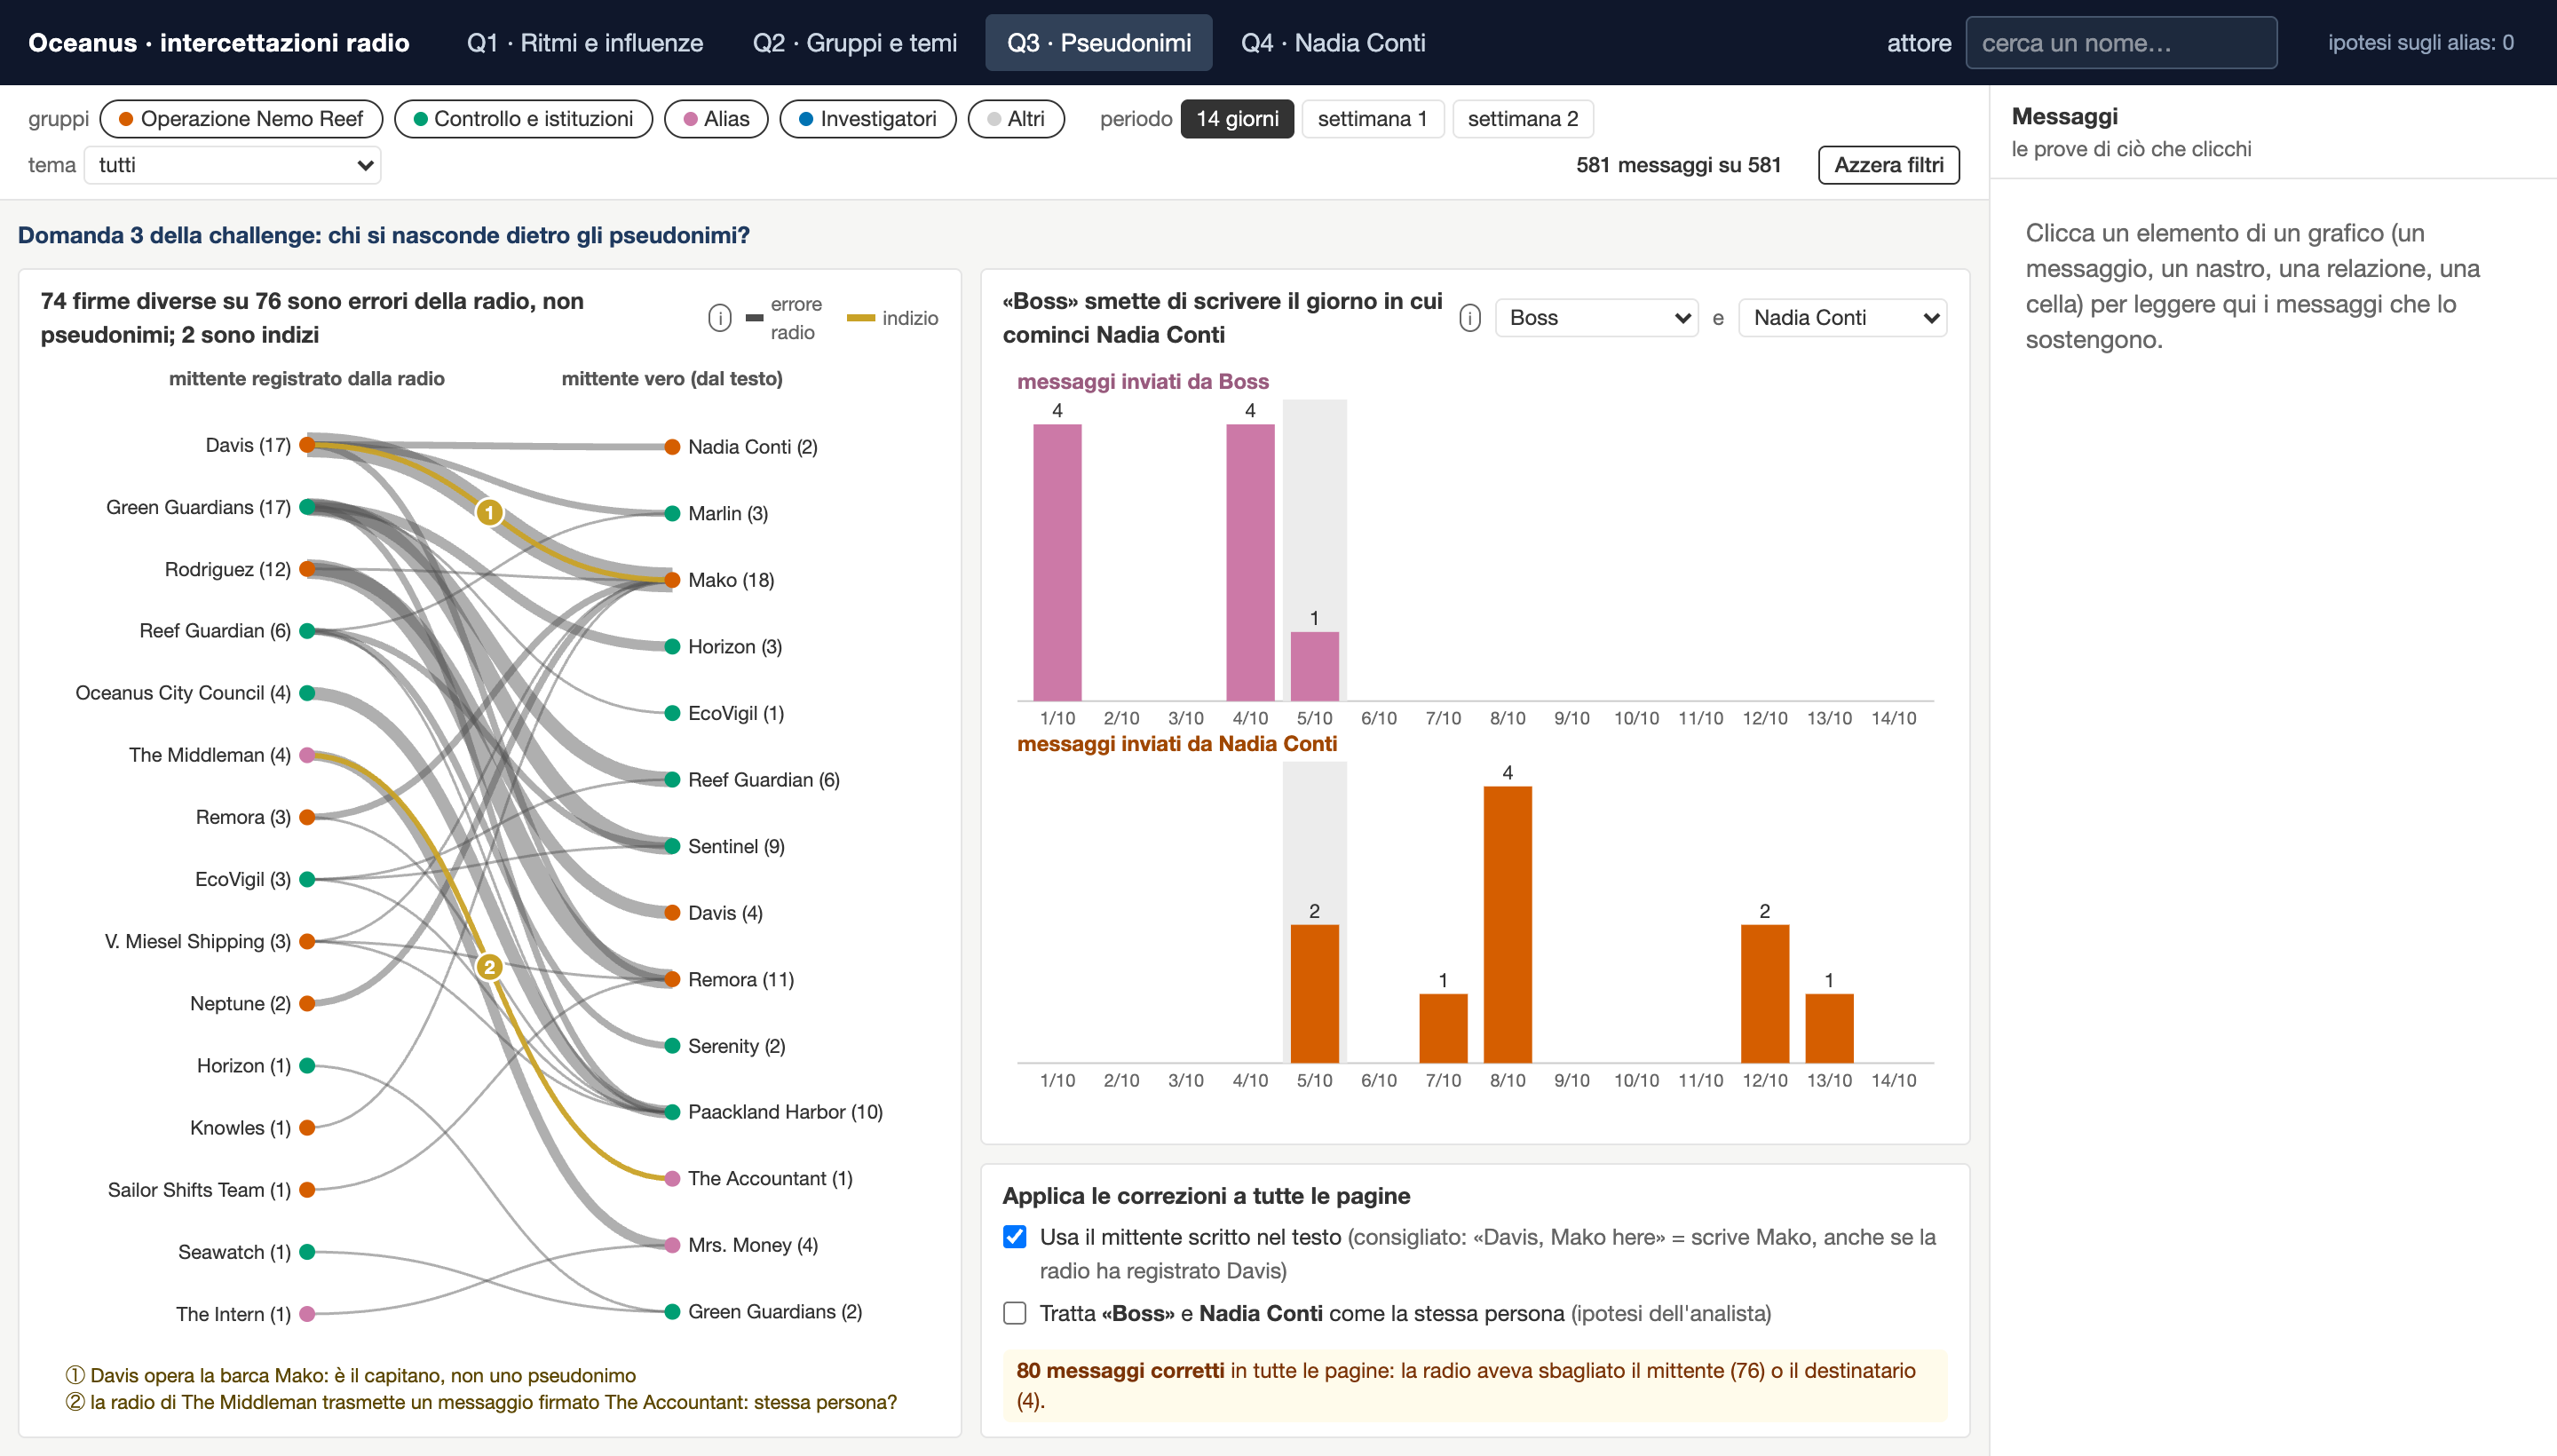
\includegraphics[width=\linewidth]{04_q3_mittenti_veri.png}
\caption{Terza pagina: a sinistra la vista originale (mittente registrato e mittente reale), a destra i
messaggi inviati ogni giorno da un alias e da un candidato e il riquadro delle correzioni.}\label{fig:p3}
\end{figure}
La pagina ha tre parti. A sinistra c'è la vista originale (sezione~\ref{sec:orig}). In alto a destra si
scelgono con due menu un alias e un candidato, per esempio Boss e Nadia Conti: il grafico mostra quanti
messaggi invia ciascuno dei due ogni giorno, l'alias sopra e il candidato sotto sulla stessa scala, e i giorni
in cui scrivono entrambi sono evidenziati in grigio. In basso a destra ci sono due caselle che valgono per
tutta l'applicazione: la prima usa il mittente scritto nel testo al posto di quello registrato dalla radio, la
seconda tratta l'alias e il candidato scelti come la stessa persona.

Prima di arrivare a questa versione avevo provato una matrice di somiglianza tra alias e candidati, basata su
interlocutori e giorni in comune: per Boss tutti i candidati avevano valori tra il 13\% e il 14\%, quindi non
aiutava a distinguerli.

\subsubsection{Q4: Nadia Conti}
\begin{figure}[!htbp]\centering
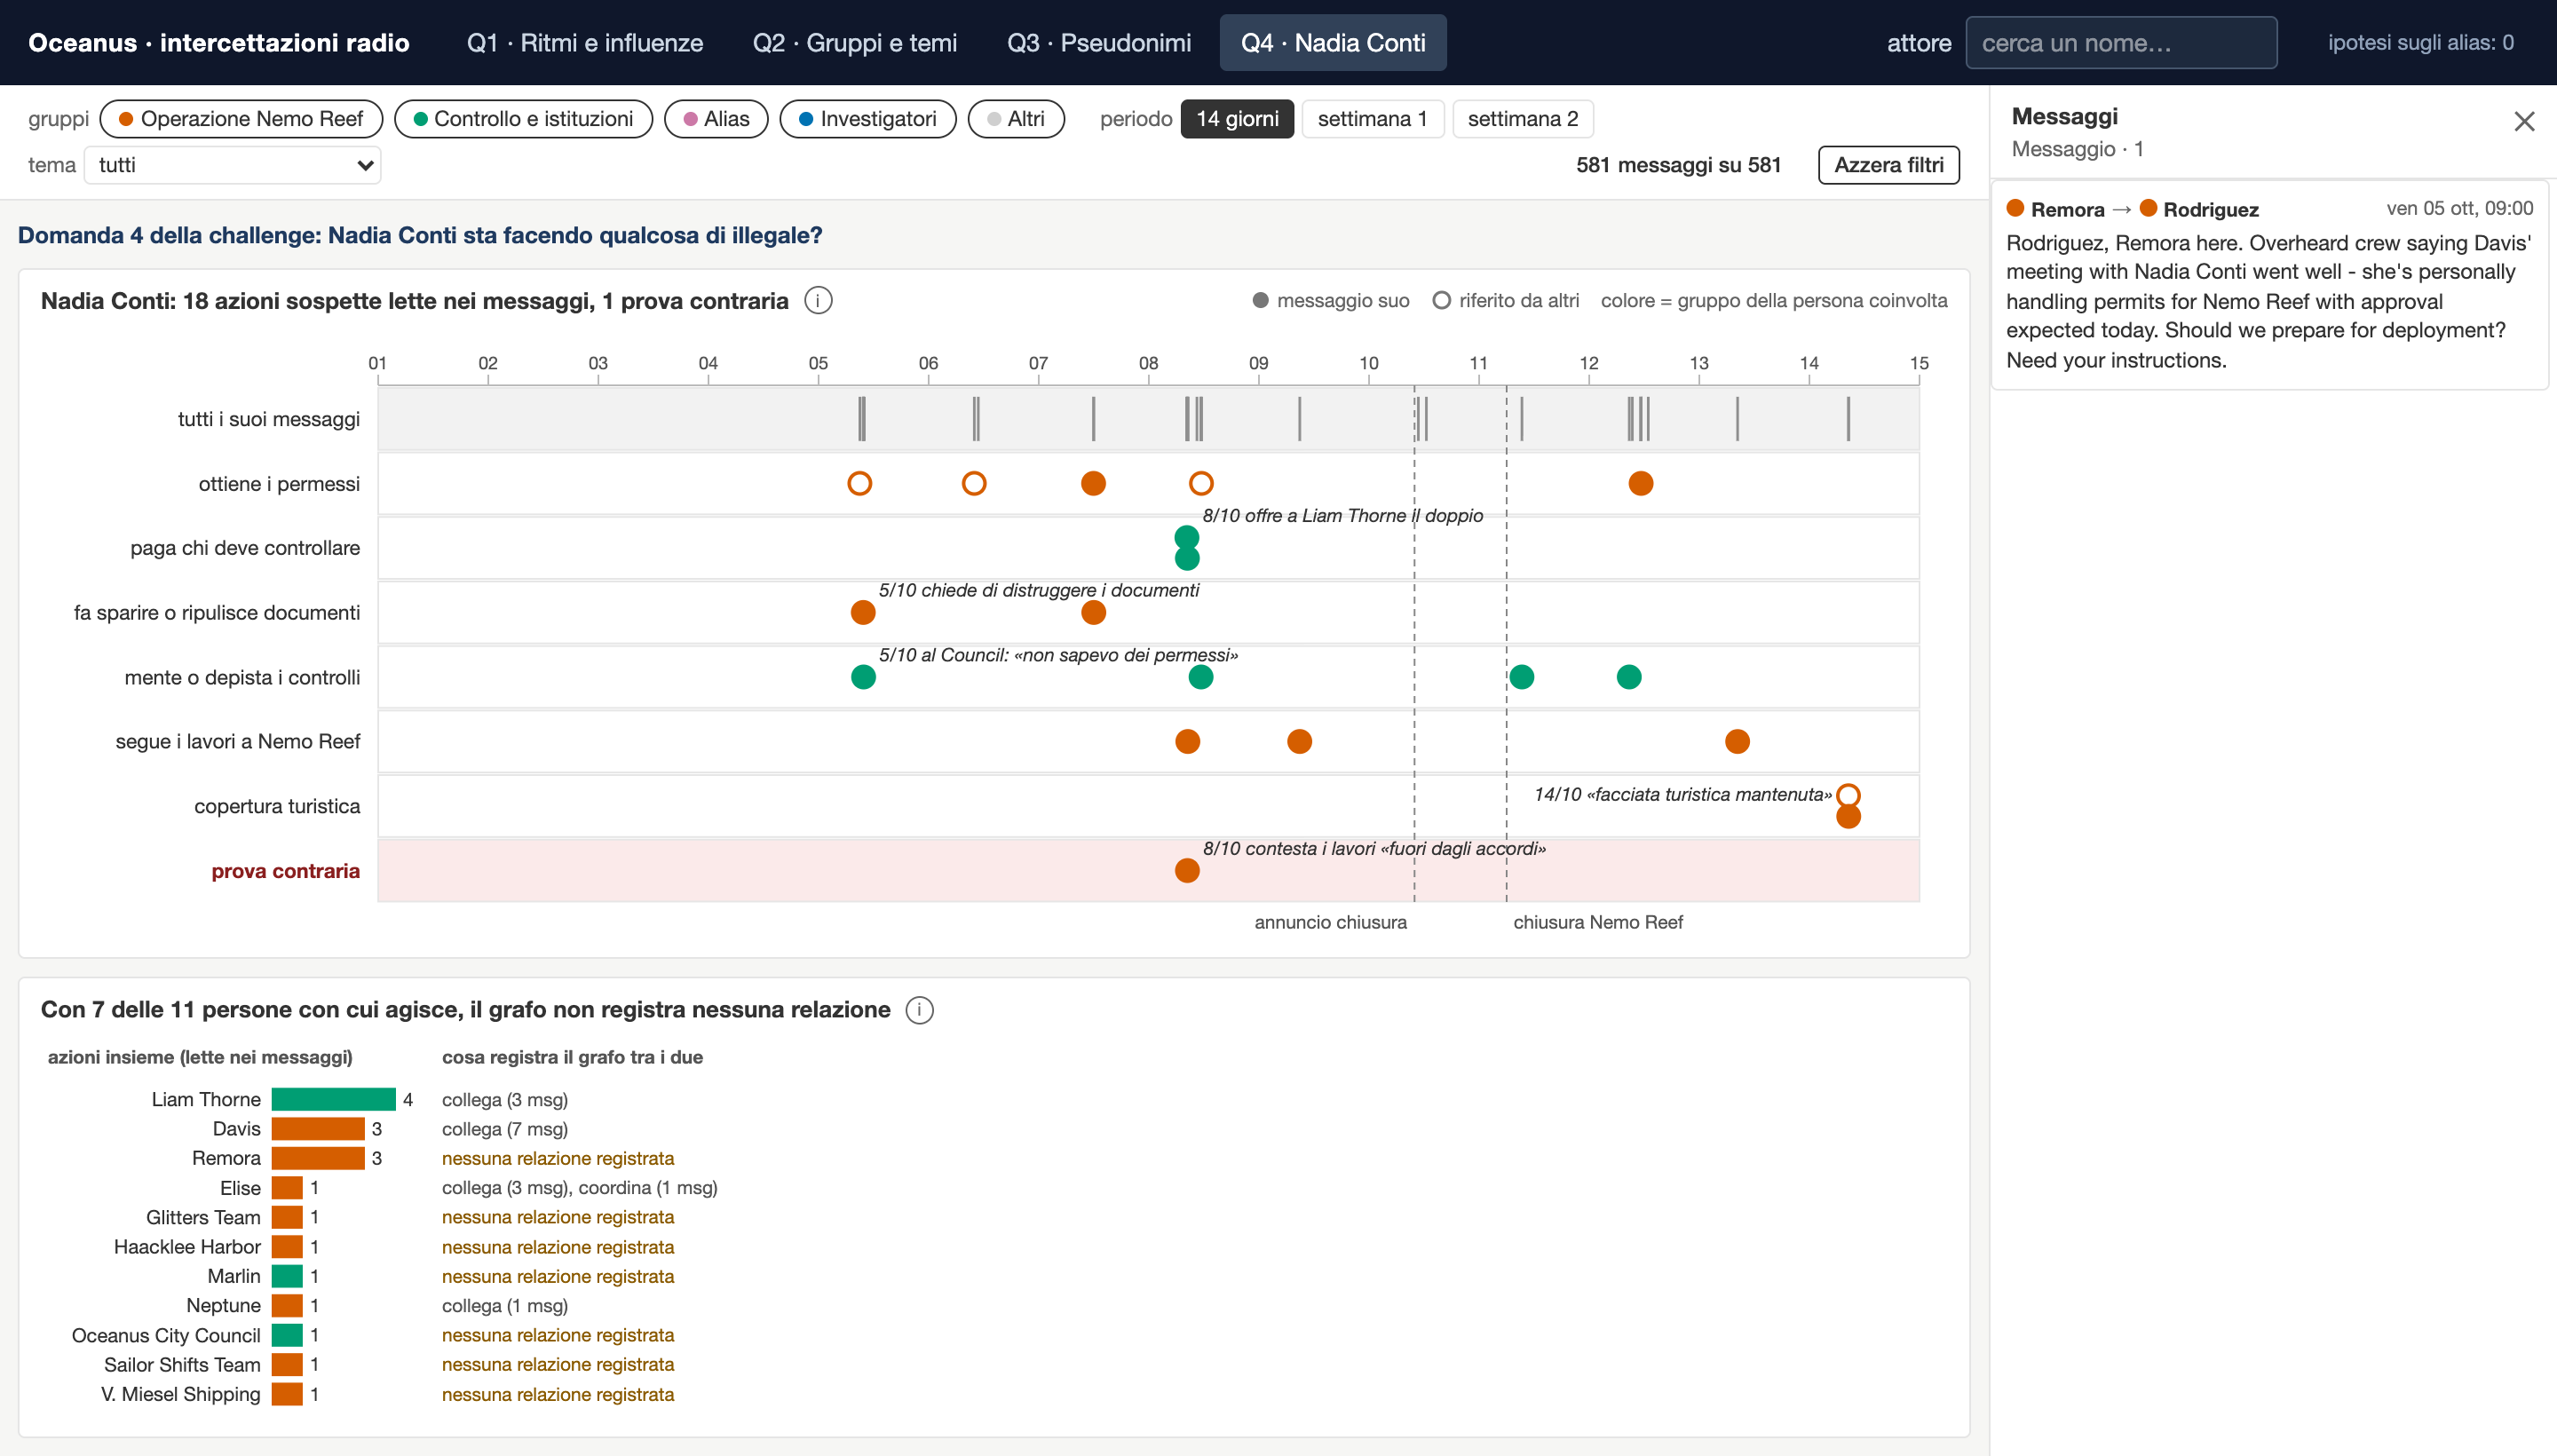
\includegraphics[width=\linewidth]{06_q4_azioni_nadia.png}
\caption{Quarta pagina: le azioni di Nadia Conti nel tempo e le persone con cui agisce; a destra il messaggio
selezionato.}\label{fig:p4}
\end{figure}
La timeline ha una riga per ogni tipo di azione (ottiene i permessi, paga chi deve controllare, fa sparire
documenti, mente o depista i controlli, segue i lavori a Nemo Reef, copertura turistica) e in fondo una riga per
la prova contraria. Il cerchio pieno indica un messaggio scritto o ricevuto da lei, quello vuoto un'azione
riferita da altri, quello tratteggiato un'azione attribuita attraverso un'ipotesi della terza pagina; il colore
è il gruppo della persona coinvolta. In cima ci sono tutti i messaggi in cui compare, e le linee tratteggiate
segnano l'annuncio della chiusura e la chiusura di Nemo Reef. Il grafico sotto elenca le persone con cui agisce
e, per ciascuna, la relazione che il grafo registra tra le due.

\subsection{La vista originale}\label{sec:orig}
La vista originale è il grafico a nastri della terza pagina. A sinistra c'è il mittente registrato dalla radio,
a destra quello scritto nel testo, e ogni nastro collega una coppia con uno spessore proporzionale al numero di
messaggi. È stata realizzata in D3 e ha quattro caratteristiche.
\begin{enumerate}
  \item Ogni discrepanza viene classificata automaticamente (mittente e destinatario invertiti, messaggio a sé
        stesso, altro). I nastri degli errori della radio sono grigi; i casi che non si spiegano come errore
        hanno un nastro separato giallo, anche quando collegano gli stessi nomi di un nastro grigio.
  \item I due nastri gialli hanno un numero e sotto il grafico c'è la loro spiegazione, ricavata dalle
        relazioni del grafo: se il mittente registrato opera la barca che firma il messaggio, la vista lo
        scrive.
  \item L'ordine dei nomi a destra è calcolato per ridurre gli incroci: ogni nome viene messo nella posizione
        media dei suoi mittenti a sinistra (metodo del baricentro) e poi vengono scambiati i nomi vicini finché
        gli incroci diminuiscono. Pesando ogni incrocio con lo spessore dei due nastri, si passa da 1031 (nomi
        ordinati per numero di messaggi) a 544. Il nastro sotto il mouse viene portato in primo piano.
  \item Le scelte fatte qui valgono per tutta l'applicazione. Se si toglie la correzione, tutte le pagine
        tornano ai dati originali della radio (cambiano 80 messaggi); se si attiva un'ipotesi su un alias,
        l'alias viene unito alla persona in tutte le viste: il nodo Boss sparisce dal grafo della seconda
        pagina, il grafico su chi attiva chi nella prima pagina viene ricalcolato e nella quarta pagina compaiono, tratteggiate,
        le azioni di Boss (Fig.~\ref{fig:ipotesi}).
\end{enumerate}
La forma del grafico è quella di un normale diagramma bipartito. La parte nuova è l'uso per verificare il
grafo: il colore indica il tipo di errore, gli indizi sono spiegati con una seconda fonte e l'analista può
decidere quali correzioni applicare e vedere subito il prima e il dopo nelle altre pagine.

\begin{figure}[!htbp]\centering
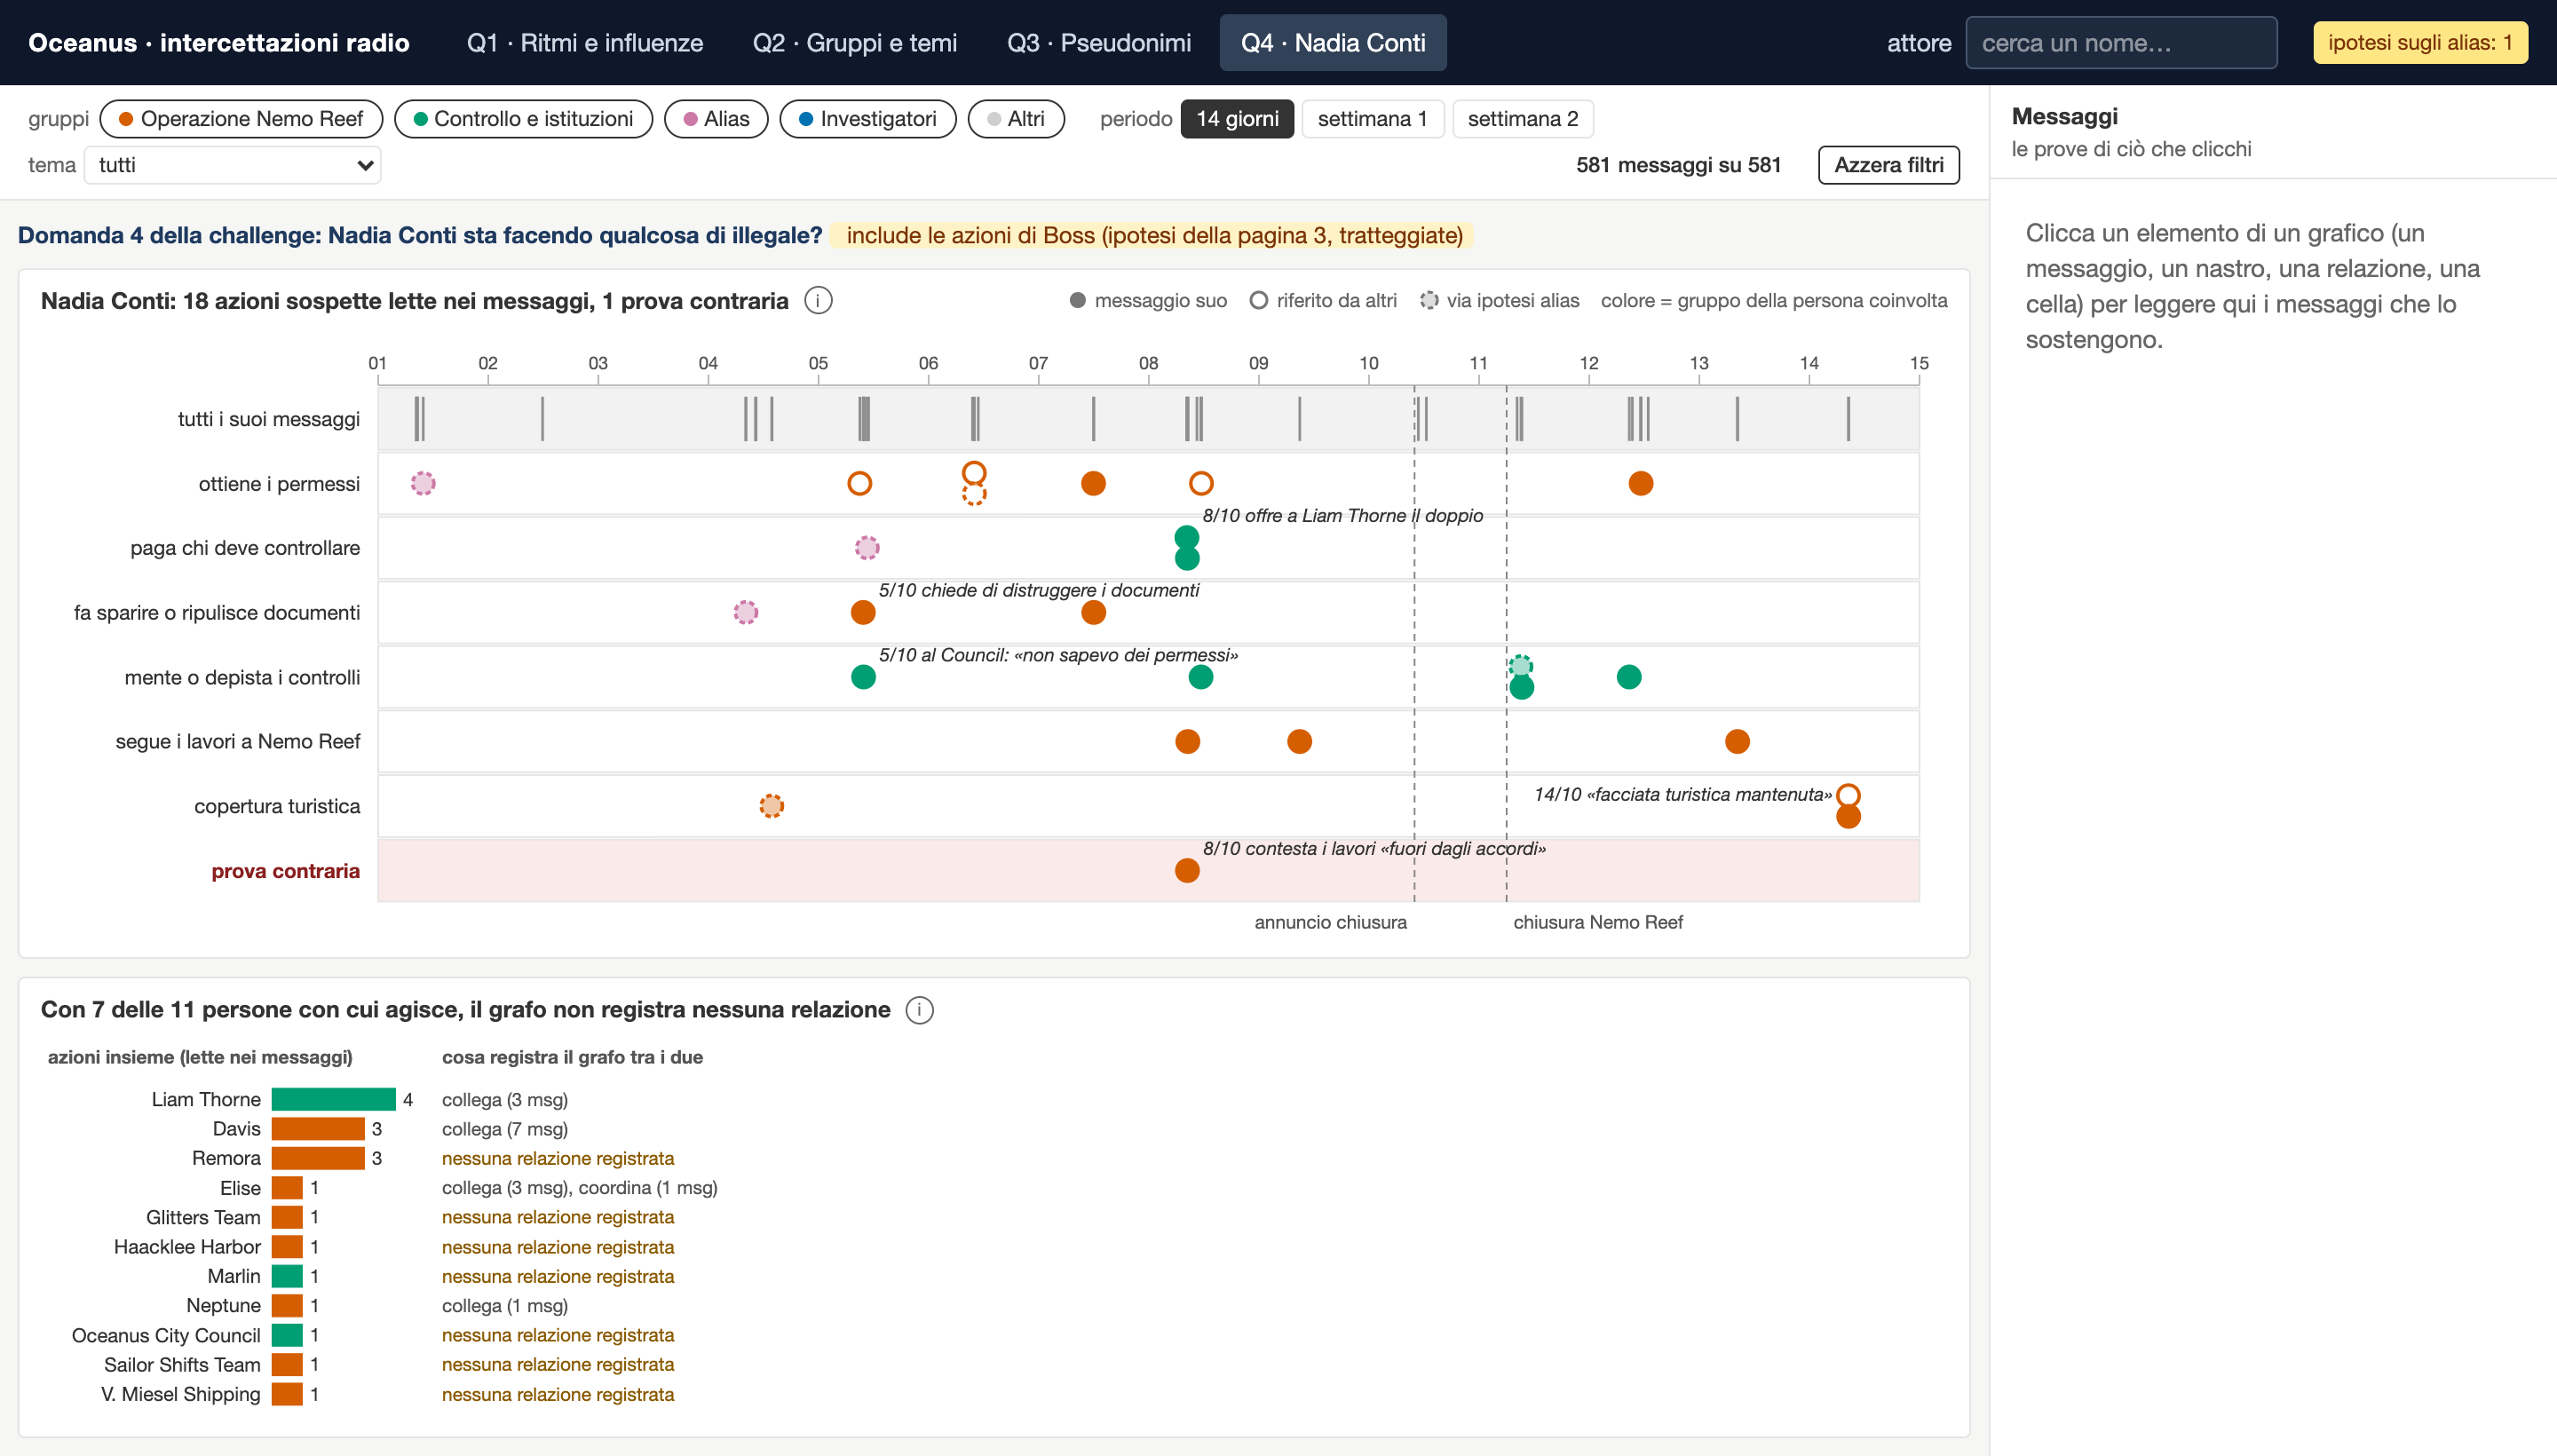
\includegraphics[width=\linewidth]{05_q3_ipotesi_boss_nadia.png}
\caption{Quarta pagina con l'ipotesi ``Boss = Nadia Conti'' attiva: le azioni di Boss compaiono tratteggiate.}\label{fig:ipotesi}
\end{figure}

\subsection{Caso d'uso: Boss e Nadia Conti}
Il giornalista parte dalla terza pagina. Il titolo della vista a nastri gli dice che 74 firme diverse su 76
sono errori della radio, quindi non deve considerarle pseudonimi. Sceglie l'alias Boss e il candidato Nadia
Conti: il titolo del grafico a barre diventa ``Boss smette di scrivere il giorno in cui comincia Nadia Conti''.
Cliccando le barre del 5 ottobre legge l'ultimo messaggio di Boss (alle 10:38) e i primi di Nadia (dalle 9:45).
Cambiando candidato vede però che anche Elise, Rodriguez e Sam scrivono solo dopo l'ultimo messaggio di Boss,
quindi questo indizio da solo non basta. Scegliendo come attore prima Boss e poi Nadia, nella quarta pagina
legge i messaggi in cui compaiono e trova due coppie di messaggi quasi contemporanei: il 6 ottobre, a un minuto di distanza, Glitters ringrazia Boss per i permessi firmati in poche ore
dal commissario Torres e Remora racconta che è stata Nadia a far firmare Torres; l'11 ottobre Liam Thorne avvisa
del ROV di EcoVigil prima Boss e, 13 minuti dopo, Nadia. A questo punto attiva l'ipotesi ``Boss = Nadia Conti''
e passa alla quarta pagina, dove le azioni di Boss si aggiungono tratteggiate a quelle di Nadia. Disattivandola
verifica che il giudizio su Nadia resta lo stesso anche senza l'ipotesi.

\subsection{Risposte alle domande della challenge}\label{sec:risposte}
\paragraph{Domanda 1.} I messaggi sono inviati solo tra le 8 e le 15, ma l'83\% degli orari citati nei testi
cade fuori da questa fascia, soprattutto tra le 5 e le 6 di mattina e tra le 21 e le 22: la radio viene usata di
giorno per organizzare attività che avvengono all'alba o di sera. Il giorno con più messaggi è l'11 ottobre (49),
il giorno della chiusura di Nemo Reef. Nella seconda settimana aumentano i messaggi su \emph{chiusura dell'area}
(+55) e \emph{attrezzature / lavori} (+51) e diminuiscono quelli sull'\emph{evento Sailor Shift} ($-28$) e su
\emph{Nemo Reef} ($-26$); il gruppo Operazione Nemo Reef invia 25 messaggi in più, gli altri gruppi meno. Per
l'influenza, per esempio, Remora viene attivata soprattutto da Mako (5 volte) e a sua volta attiva Rodriguez
(9 volte); Nadia Conti viene attivata più spesso da Davis.

\paragraph{Domanda 2.} I gruppi sono quattro: Operazione Nemo Reef (Nadia Conti, Davis, Elise, le barche Mako,
Remora e Neptune, V.\ Miesel Shipping, lo staff di Sailor Shift), Controllo e istituzioni (Oceanus City Council,
porti, Green Guardians, barche di sorveglianza, Liam Thorne), Alias e Investigatori. Gli alias parlano
soprattutto tra loro (75\% dei loro messaggi) e parlano di soldi e pagamenti molto più degli altri gruppi (49\%
contro al massimo l'8\%). Controllo e istituzioni parla soprattutto di Nemo Reef (64\%), gli investigatori di
ambiente (50\%) e lavori (47\%), l'Operazione di permessi (39\%) e lavori (36\%). Confrontando i collegamenti dei
messaggi con quelli delle relazioni si vedono legami che il grafo dello stagista non contiene.

\paragraph{Domanda 3.}\label{sec:q3} Le 74 firme dovute a errori della radio non indicano pseudonimi. I due casi
rimanenti sono indizi. Nel primo la radio registra Davis come mittente di un messaggio firmato Mako, e il grafo
dice che Davis opera la barca Mako (13 messaggi a sostegno): Davis è quindi il capitano che parla a nome della
barca. Nel secondo, il 13 ottobre, la radio di The Middleman trasmette un messaggio firmato The Accountant:
potrebbero essere la stessa persona, ma si basa su un solo messaggio e resta un'ipotesi aperta. L'ipotesi più
sostenuta è che dietro Boss ci sia Nadia Conti, per gli indizi descritti nel caso d'uso: Boss smette di scrivere il
giorno in cui lei comincia, hanno contatti in comune (Liam Thorne e V.\ Miesel Shipping) e due coppie di messaggi
attribuiscono gli stessi fatti a entrambi. Non è una prova, per cui nell'applicazione resta un'ipotesi che
l'analista sceglie di attivare. Per The Intern, The Lookout, Mrs.\ Money e The Middleman i messaggi sono
distribuiti su tutto il periodo e non ci sono indizi sufficienti per associarli a una persona.

\paragraph{Domanda 4.} Secondo i messaggi Nadia Conti è coinvolta in attività illegali. Il 5 ottobre chiede ad
Haacklee Harbor di annullare il corridoio speciale e di distruggere i documenti, e quattro minuti dopo dice al
Council di non sapere nulla dei permessi. Il 7 ottobre chiede a Davis di creare ``una traccia di carte pulita''.
L'8 ottobre offre a Liam Thorne il doppio perché l'Harbor Master ``collabori'' e Liam le conferma di aver
spostato le pattuglie. Tra l'8 e il 13 ottobre segue le attrezzature per le fondazioni, dicendo di restare
``sotto i radar'', e la documentazione del permesso \#CR-7844. Il 14 ottobre Remora le comunica che la facciata
turistica è mantenuta. In totale sono 18 azioni, 14 in messaggi scritti o ricevuti da lei e 4 riferite da altri.
C'è anche una prova contraria: l'8 ottobre contesta a Neptune dei lavori di fondazione ``fuori dagli accordi''.
Può essere un disaccordo reale sui lavori o un modo per coprirsi, ma non cambia quanto emerge su permessi e
pagamenti. Il risultato non dipende dall'ipotesi su Boss, le cui 6 azioni compaiono solo se l'ipotesi è attiva.
Infine, per 7 delle 11 persone con cui agisce il grafo non registra nessuna relazione: senza leggere i testi
questi collegamenti non si vedrebbero.

%---------------------------------------------------------------------
\section{Limiti e conclusioni}
%---------------------------------------------------------------------
L'applicazione ha alcuni limiti:
\begin{itemize}
  \item i temi sono trovati con parole chiave, quindi ci possono essere falsi positivi o messaggi non
        riconosciuti;
  \item le azioni sospette le ho segnate a mano solo per Nadia Conti e Boss; se nella quarta pagina si sceglie
        un altro attore, si vedono i suoi messaggi ma non le azioni;
  \item il grafico su chi attiva chi conta quante volte un attore scrive entro 15 minuti dopo aver ricevuto un
        messaggio: mostra chi viene prima nel tempo, ma non prova che uno dia ordini all'altro;
  \item per gli pseudonimi nessun indizio calcolato è sufficiente da solo, e le ipotesi restano una scelta
        dell'analista;
  \item i gruppi dipendono dall'algoritmo usato (con un altro metodo potrebbero cambiare un po'), e i loro nomi li ho scelti io;
  \item la correzione dei mittenti presuppone che la firma nel testo sia vera;
  \item l'interfaccia è pensata per uno schermo di almeno 1440$\times$820 pixel.
\end{itemize}

In conclusione, l'applicazione permette di rispondere alle quattro domande partendo dai ritmi delle
comunicazioni, passando per i gruppi e gli pseudonimi fino al caso di Nadia Conti. Il punto più importante
emerso dal lavoro è la verifica dei mittenti: buona parte delle firme ``sospette'' erano errori della radio, e
correggerle cambia i risultati di tutte le pagine. Come sviluppi futuri si potrebbero estendere la codifica delle
azioni agli altri attori, permettere ipotesi anche tra due alias (come The Middleman e The Accountant) e
sostituire le parole chiave con un modello di classificazione dei temi.

\end{document}
